
\section{Preliminaries}
\label{sec:background}
\newcommand{\satisfies}{\vdash_{\!\!s}}
\newcommand{\nsatisfies}{\nvdash_{\!\!s}}
\newcommand{\bool}[0]{\mathit{bool}}
\newcommand{\reach}[0]{\mathit{R}}
\newcommand{\ite}[3]{\mathit{if}\ {#1}\ \mathit{then}\ {#2}\ \mathit{else}\ {#3}}
\newcommand{\nondetcov}{\text{\sc Nondet-Cov}}
\newcommand{\mutcov}{\text{\sc Mutant-Cov}}

\subsection{Models, Requirements, and Provability}

We define \emph{provability} of a requirement with respect to a model independent of a particular proof system.  We define the implementation model as a set of formulas $\Gamma$  and the set of requirements $\Delta$.
Then given $\Gamma' \subseteq \Gamma$ and $\delta \in \Delta$, we use the notation $\Gamma' \vdash \delta$ to mean that $\delta$ is \emph{provable} given the set $\Gamma'$.  We assume that the provability relation $\vdash$ is monotonic on the subset relation over $\Gamma$, that is, if $\Gamma'' \subseteq \Gamma' \subseteq \Gamma$ and $\Gamma'' \vdash \delta$, then $\Gamma' \vdash \delta$.  The monotonicity of the satisfaction relation means that, unless {\em all} elements of the implementation $\Gamma$ are required for a proof, there are multiple implementation sets $\Gamma'' \subset \Gamma' \subset \ldots \subset \Gamma$ that can satisfy a given requirement $\delta$.  In an abuse of notation, we write $\Gamma' \vdash \Delta$ to mean the conjunction of all requirements in $\Delta$: $\Gamma' \vdash \bigwedge \Delta$.

\subsubsection{Example: Transition Systems}
\label{sec:ts}
We can straightforwardly instantiate our abstract model over a transition system for proving safety properties.  Given a state space $S$, a transition system $(I,T)$ consists of an initial state predicate $I : S \to \bool$ and a transition step predicate $T : S \times S \to \bool$. We define the notion of reachability for $(I, T)$ as the smallest predicate $\reach : S \to \bool$ which satisfies the following formulas:
\begin{gather*}
  \forall s.~ I(s) \Rightarrow \reach(s) \\
  \forall s, s'.~ \reach(s) \land T(s, s') \Rightarrow \reach(s')
\end{gather*}
A safety property $P : S \to \bool$ is a state predicate. A safety property $P$ holds on a transition system $(I, T)$ if it holds on all reachable states, i.e., $\forall s.~ \reach(s) \Rightarrow P(s)$, written as $\reach \Rightarrow P$ for short. When this is the case, we write $(I, T)\vdash_{T} P$, for provability within the transition system.  We assume the transition relation of the system has the structure of a top-level conjunction. This assumption gives us a structure that we can easily manipulate. Given $T(s, s') = T_1(s, s') \land \cdots \land T_n(s, s')$ we will write $T = T_1 \land \cdots \land T_n$ for short. By further abuse of notation we will identify $T$ with the set of its top-level conjuncts. Thus we will write $x \in T$ to mean that $x$ is a top-level conjunct of $T$; or, equivalently, $\Gamma = \{T_1, T_2, \ldots, T_n\}$ and $\Delta = \{P\}$ in our abstract model.

Such a transition system can easily encode our example model in Section~\ref{sec:example}.  We assume each equation defines a conjunct within the transition system which we will denote by the variable assigned, so $\Gamma = \{$ {\small \texttt{a1\_below, a2\_below, a1\_above, a2\_above, below, above\_hyst}} $\}$.
%\footnote{In the example in Section \ref{sec:example}, $\Gamma = \{{\tt P}, {\tt x}, {\tt c1}, {\tt c2}, {\tt c3}, {\tt r1}, {\tt r2}\}$ and $\Delta = \{{\tt P}\}$.}

%Such transition systems can represent either finite or infinite state systems, depending on the state space $S$.

%We will write $S \subseteq T$ to mean that all top-level conjuncts of $S$ are top-level conjuncts of $T$. We will write $T \setminus \{x\}$ to mean $T$ with the top-level conjunct $x$ removed.


%\paragraph{Applying Provability to Transition Relations and Safety Properties}

%\mike{To do: add a few paragraphs on instantiating the formal model for transition systems and model checking (a la IVCs), then further elaborate it for Netlists (a la Chockler and Kroening).}

%\mike{We could cover tableau methods here, but these are overly restrictive}

\subsection{Requirements Coverage and Mutations}
The goal of a coverage metric is usually to assign a numeric score that describes how well requirements cover the design.  The majority of the work in requirements coverage metrics has focused on {\em mutations}, which are ``atomic'' changes to the design, where the set of possible mutations depends on the notation that is used.  A mutant is ``killed'' if one of the requirements that is satisfied by the original design is violated by the mutated design~\cite{chockler_coverage_2003,chockler2001practical,chockler2010coverage,Kupferman:2006:SCF,kupferman_theory_2008}.  There are Many different kinds of mutations that have been proposed, primarily focused on checking sequential bit-level hardware designs.  For these designs, {\em State-based} mutations flip the value of one of the bits in the state.  There are several variations depending on whether the flip is performed on a single state within a Kripke structure~\cite{hoskote1999coverage}, or in the description of the signal in the transition relation of the circuit~\cite{chockler2001practical}.  {\em Logic-based} mutations fix the value of a bit to constant zero or one, and can be used to determine whether requirements can find stuck-at faults.  {\em Syntactic} mutations~\cite{chockler_coverage_2003} remove states in a control flow graph representation of hardware.  Similarly, for software, it is possible to apply any of the ``standard'' source code mutation operators used for software testing~\cite{Andrews06:mutation} towards requirements coverage analysis.  Some examples of software mutations are:
\begin{enumerate}
    \item Replace an integer constant C by one of $\{0, 1, -1, C + 1, C - 1\}$.
    \item Replace an arithmetic, relational, logical, bitwise logical, increment/decrement, or arithmetic-assignment operator by another operator from the same class.
    \item Negate the decision in an if or while statement
    \item Delete a statement
\end{enumerate}


For our abstract model, we assume each element $\gamma \in \Gamma$ has a set of possible mutations associated with it.  Depending on the modeling formalism used, this may be the value of a gate or signal or an expression within a statement in a program.  We will further assume the existence of a mutation function $f_{m}$ that, given a model element, will return a finite set of mutations for that element.  We can then define the set of mutant models $M$ as follows:
\[
    M = \{ \gamma \in \Gamma, m \in f_{m}(\gamma)\ |\ \Gamma - \{\gamma\} \cup \{m\} \}
\]

\noindent and then define the mutation score for a set of requirements $\Gamma$ in the standard way:

\begin{definition} {\emph{Generalized mutation coverage.} } \\
\[
   \mutcov = \frac{ | \{m \in M(\Gamma)~|~ m \nvdash \Delta\} |}{|M(\Gamma)|}
\]
\end{definition}

%\mike{Do we want these parameterized?  We could just assume Gamma and Delta}

In our example in Figure~\ref{fig:asw}, applying the software mutations from~\cite{Andrews06:mutation} would involve manipulating the constants used in the definitions of \texttt{a1\_below, a2\_below, a1\_above, a2\_above}, swapping 'or' and 'and' in the definition of \texttt{below, above\_hyst}, or negating the conditions in the if/then/else statements.  Even for this small model, note that there are a large number of possible mutations: 57 given the set defined above, and that this number increases rapidly with the size of the program and the chosen set of mutations.


%\mike{Illustrate on running example here.}

Of particular interest is the mutation that replaces a computed variable ({\em signal} in hardware) with a ``fresh'' input; this mutation is called a {\em nondeterminism mutation} with a coverage metric called (\nondetcov)~\cite{chockler2010coverage} and is discussed in~\cite{Kupferman:2006:SCF,kupferman_theory_2008,chockler2010coverage}.  If we use an equational transition system to assign the variables, then performing \nondetcov\ coverage an isomorphic operation to removing the defining equation from the set $\Gamma$ and checking whether provability is preserved.  In this case, we can dispense with the set $M$ and compute a mutation score much more simply:

\begin{definition} {\emph{Nondeterministic coverage.} }
\[
   \nondetcov = \frac{ | \{\gamma \in \Gamma~|~ \Gamma - \{\gamma\} \nvdash \Delta\} |}{|\Gamma|}
\]
\end{definition}

\noindent In one sense, the nondeterminism mutation is the {\em strongest} mutation because it introduces the most additional behaviors into the model, that is, any execution sequence constructed by modifying the assigning equation is also an execution sequence for a nondeterministic mutation.  Equivalently, given a set of universal properties, it is the easiest mutation to ``kill''.  For our example in Figure~\ref{fig:asw}, this mutation would lead to 10 mutations, one for each equation in the model.

%\mike{Illustrate on running example here}

\iffalse
\subsection{Requirements Coverage and Structural Testing}
\mike{not sure we need this...if so, we need to accurately characterize test obligations as a function from elements in $\Gamma$}
In {\em black-box} testing, one is interested in creating a suite of tests from requirements that adequately exercise the behavior
of a software system without regard to the internal structure of the implementation.  This is the preferred style of testing in
safety-critical domains and is advocated by standards such as DO-178B~\cite{RTCA:DO-178B}.  The adequacy of such test suites are usually inferred by examining different coverage metrics on an executable artifact, either source code~\cite{Bezier90:TestingBook,MCDCPaper} or software models~\cite{Ammann99:SpecBasedCoverageMetric,Sanjai03:dissertation}.  If the tests are not sufficient to cover the structure of the code, then either additional tests are derived from existing requirements, or (often) additional requirements are created to describe the additional functionality that is not covered by any tests.

Common metrics used for test coverage measurement are {\em statement}, {\em decision}, and {\em modified condition/decision coverage (MCDC)}.  In this section, we use the rigorous MCDC metric to measure coverage.  \mike{Define MCDC}.

It is straightforward to define coverage in a way that is parametric to the particular test metric that is used.  Given a set $\Theta$ of all possible tests and $\Phi$ the set of all {\em test obligations} induced by the test metric over the model, we define three functions.  The first, $R_m : \Delta \rightarrow 2^\Theta$, defines the set of tests furnished for each requirement.  The second, $E_m : \Gamma \rightarrow 2^\Phi$ defines the test obligations associated with each model element.  The third, $T_m : \Theta \rightarrow 2^\Phi$, defines the obligations that are covered by the test.  Then coverage can be defined as: $$\frac{|\bigcup_{t \in T} T_m (t)|}{|\Phi|}$$.


%Formally, irrespective of the metric used, given $T$ the set of all tests, and the user furnishes test cases associated with each requirement: . Coverage for a given test is measured using a function that maps tests to model elements  as follows \cite{chelenski1994oapplicability, schuler_assessing_2011, murugesan2015we}: $$\frac{|\bigcup_{t \in T} T_m (t, \Gamma)|}{|\Gamma|}$$

%
%\mike{revise}
%

A common problem with this metric is masking:
the effect of a change in a variable cannot be observed in the output. To illustrate, consider the example in Fig. \ref{fig:ex}; suppose we are provided with
test suite \{\{{\tt in1} = \emph{true}, {\tt in2} = \emph{false}\},
\{{\tt in1} = \emph{false}, {\tt in2} = \emph{false}\}\}. The change in the value of
{\tt in1} is masked by {\tt c1}. This problem causes the coverage method reports something covered
while it actually does not affect the output at all.



%\noindent In the following sections, we will examine other possible scoring mechanisms based on minimal provability, and contrast them against testing and vacuity-based metrics.

%\begin{figure}[htb]
%\begin{center}
%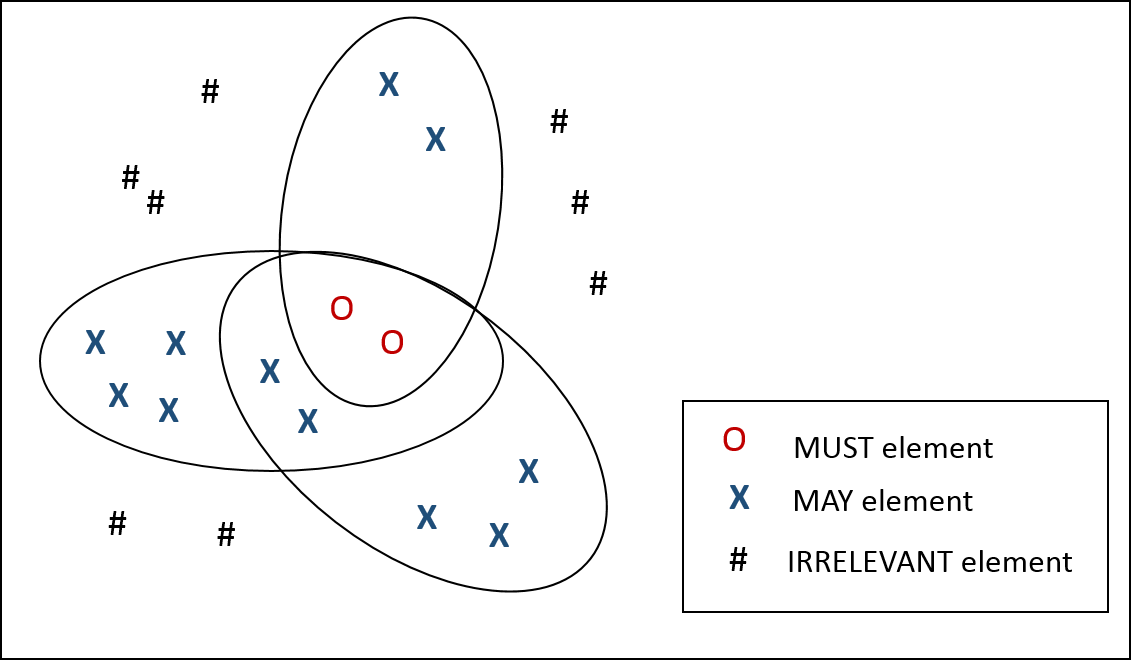
\includegraphics[width=\columnwidth]{figs/may_must.png}
%\caption{A visual example of partitioning the implementation model}\label{fig:maymust}
%\end{center}
%\end{figure}

\iffalse
In light of this intuition, we define existing coverage notions in the literature, which are based on the idea of \emph{mutation}. Then, later, we explore some novel notions of coverage based on the idea of support sets.  More formally, mutation, denoted by $f_m$, is a relation that maps $\Gamma$ to set $S \subset \Gamma$ (written as $f_m (S)$). The range of $f_m$ for $\Gamma$ is denoted by $M$.

In general, requirements completeness can be defined with regard to the notion of \emph{coverage}. In fact, the way that coverage is formalized plays a key part in the strength/ effectiveness of a method for the assessment of completeness. Requirements completeness can be judged on a fraction called \emph{coverage score}, the closer to 1 the score is, the more complete the specification is.

\begin{definition}{\emph{Coverage:}}
  \label{def:coverage}
   Any notion of coverage can be formalized as a function $\psi$ such that,
   $\forall r \in \Delta, \varphi \in \Gamma$, if $\varphi$ is covered by $r$ then $\psi (r, \varphi) = true$, denoted by $\psi (r) \preccurlyeq \varphi$, otherwise  $\psi (r, \varphi) = false$, denoted by $\psi (r) \nprec \varphi$.
\end{definition}

\begin{definition} {\emph{Coverage based on single mutation \cite{chockler2010coverage, chockler_coverage_2003}:}}
  \label{def:coverage1}
   $\forall r \in \Delta$,
   $\varphi \in \Gamma$,
   $\psi (r) \preccurlyeq \varphi$
   iff $\Gamma \vdash r$ and
   $f_m (\Gamma \setminus \{ \varphi \}) \nvdash r$. Otherwise, $\psi (r) \nprec \varphi$.
\end{definition}

For the sake of simplicity, we refer to the coverage function
formalized in Definition \ref{def:coverage1} as $\psi_{sm}$.
Back to our example, $\psi_{sm}$ only considers {\tt P} and {\tt c3} as covered in the model shown in Fig. \ref{fig:ex}.

Using $\psi_{sm}$, the coverage score of specification $r$ is computed by $$\frac{\sum_{\varphi \in \Gamma} f_m (\Gamma \setminus \{ \varphi \}) \nvdash r}{|\Gamma|}$$
Usually, a mutation is an atomic change to the design whose effect is not masked by other modifications, which means simultaneous mutations may result in masking the changes. However,
it is possible to define the coverage notion with regard to all possible mutations, although it would be also very expensive and impractical \cite{chockler2001practical}. \ela{Mike, is the citation correct?}.
For a coverage function based on all mutations, the coverage score is calculated by
$$ \frac{\sum_{S \in M} f_m (S) \nvdash r}{|\Gamma| |M|}$$
\fi
\fi



